\documentclass[11pt,a4paper]{article}

\usepackage[T1]{fontenc}
\usepackage[utf8]{inputenc}
\usepackage[english]{babel}
\usepackage{lmodern}
\usepackage{microtype}
\usepackage[margin=2.5cm]{geometry}
\usepackage{xcolor}
\usepackage{graphicx}
\usepackage{booktabs}
\usepackage{tabularx}
\usepackage{enumitem}
\usepackage{tikz}
\usetikzlibrary{positioning,arrows.meta,shapes.multipart}
\usepackage[most]{tcolorbox}
\usepackage{fancyhdr}
\usepackage{titlesec}
\usepackage[hidelinks]{hyperref}

\definecolor{accent}{HTML}{1F4E79}
\definecolor{tipbg}{HTML}{EAF2FB}
\definecolor{warnbg}{HTML}{FDF1E6}
\definecolor{warnfr}{HTML}{C0611B}

\titleformat{\section}{\Large\bfseries\color{accent}}{\thesection}{1em}{}
\titleformat{\subsection}{\large\bfseries\color{accent}}{\thesubsection}{1em}{}

\setlist{itemsep=2pt,topsep=4pt}
\setlength{\parindent}{0pt}
\setlength{\parskip}{6pt}

\pagestyle{fancy}
\fancyhf{}
\fancyhead[L]{\small\color{gray}Thin Film Logbook}
\fancyhead[R]{\small\color{gray}User manual}
\fancyfoot[C]{\small\thepage}
\renewcommand{\headrulewidth}{0.4pt}

% UI elements: buttons, menu entries, field names
\newcommand{\ui}[1]{\textsf{\textbf{#1}}}
\newcommand{\menu}[1]{\textsf{#1}}
\newcommand{\sid}[1]{\texttt{#1}}

\newtcolorbox{tip}{colback=tipbg,colframe=accent,boxrule=0.5pt,arc=2pt,
  left=6pt,right=6pt,top=4pt,bottom=4pt,fonttitle=\bfseries,title=Tip}
\newtcolorbox{careful}{colback=warnbg,colframe=warnfr,boxrule=0.5pt,arc=2pt,
  left=6pt,right=6pt,top=4pt,bottom=4pt,fonttitle=\bfseries,title=Careful}

\title{\color{accent}\textbf{Thin Film Logbook}\\[4pt]\large User manual}
\author{}
\date{\today}

\begin{document}

\maketitle
\thispagestyle{empty}

\begin{abstract}
The Thin Film Logbook is a web application for recording what happens to
every sample in the lab: where it came from, each process step
(deposition, annealing, implantation, \ldots), each analysis (XRD, RBS,
SEM, \ldots), and the photos and data files that go with them. This manual
explains how to use it day to day. Section~\ref{sec:admin} covers the
extra tasks for administrators, and Section~\ref{sec:install} how to run
and back up the server.
\end{abstract}

\tableofcontents
\newpage

%=====================================================================
\section{Getting started}
%=====================================================================

\subsection{Opening the logbook}

The logbook runs on a lab computer and is opened in any web browser, on a
computer or a phone, at the address the administrator gives you, for
example \texttt{http://10.10.13.172:8000}. You need to be on the lab
network.

\subsection{Your account}

There is no self-registration: an administrator creates your account. You
receive an email with your username and a temporary password (or the
administrator gives them to you).

\begin{enumerate}
  \item Sign in with the username and temporary password.
  \item You are asked to choose a new password.
  \item You are asked for your \ui{Name} (shown as the researcher on your
        samples) and your \ui{Initials}: 2--4 letters, unique in the lab.
        Your initials go into your sample IDs, e.g.\ \sid{ASS-2026-001}.
\end{enumerate}

\begin{careful}
Choose your initials carefully. Once you have samples, only an
administrator can change them, and existing sample IDs never change.
\end{careful}

If you forget your password, use \ui{Forgot password?} on the sign-in page:
you receive an email with a one-time sign-in link. You can change your
password and name at any time from your profile (click your name at the
bottom of the sidebar).

\subsection{Finding your way around}

The sidebar on the left (a menu button on phones) has:

\begin{center}
\begin{tabularx}{\linewidth}{@{}lX@{}}
\toprule
\menu{Samples}     & All samples in the lab, newest first. \\
\menu{Search}      & Filter, group, share and export samples. \\
\menu{Substrates}  & The shared library of substrates samples are made from. \\
\menu{Projects}    & Collaboration projects with other institutions. \\
\menu{New Sample}  & Create a sample. \\
\menu{Suggestions} & Send an idea, a problem or a question to the administrators. \\
\menu{Inbox}, \menu{Configurations} & Administrators only (Section~\ref{sec:admin}). \\
\bottomrule
\end{tabularx}
\end{center}

At the bottom of the sidebar are the \ui{PT / EN} language switch and the
moon/sun button for dark mode. Technical terms (technique names, units,
dropdown values) stay in English in both languages.

%=====================================================================
\section{Key ideas}
%=====================================================================

\begin{center}
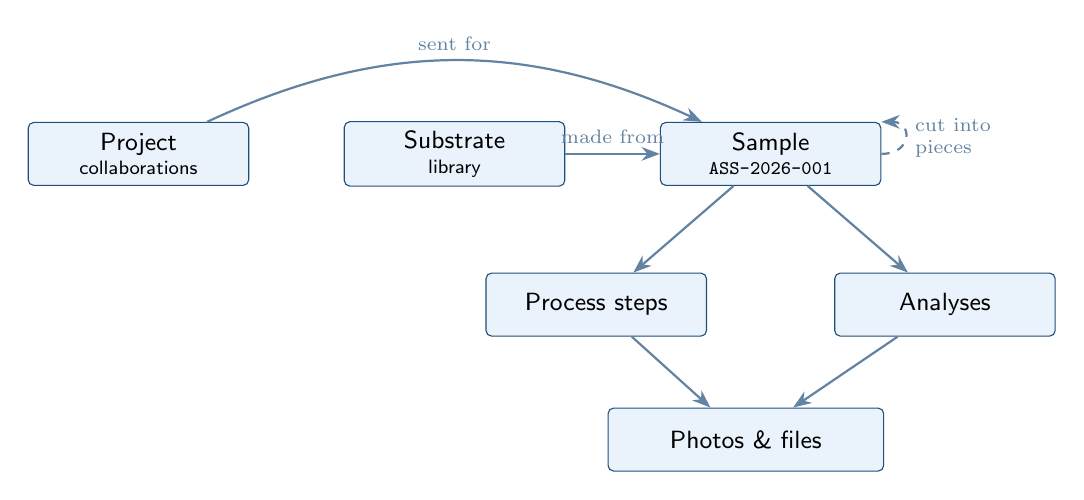
\begin{tikzpicture}[
  box/.style={draw=accent,rounded corners=2pt,fill=tipbg,minimum width=2.8cm,
              minimum height=0.8cm,font=\sffamily\small,align=center},
  arr/.style={-{Stealth},thick,accent!70}]
  \node[box] (sub) {Substrate\\[-2pt]\scriptsize library};
  \node[box,right=1.2cm of sub] (sam) {Sample\\[-2pt]\scriptsize\texttt{ASS-2026-001}};
  \node[box,left=1.2cm of sub, yshift=0cm] (prj) {Project\\[-2pt]\scriptsize collaborations};
  \node[box,below left=1.1cm and -0.6cm of sam] (stp) {Process steps};
  \node[box,below right=1.1cm and -0.6cm of sam] (ana) {Analyses};
  \node[box,below=0.9cm of stp,xshift=1.9cm,minimum width=3.5cm] (att) {Photos \& files};
  \draw[arr] (sub) -- node[above,font=\scriptsize]{made from} (sam);
  \draw[arr] (prj) to[bend left=25] node[above,font=\scriptsize]{sent for} (sam);
  \draw[arr] (sam) -- (stp);
  \draw[arr] (sam) -- (ana);
  \draw[arr] (stp) -- (att);
  \draw[arr] (ana) -- (att);
  \draw[arr,dashed] (sam.east) to[out=0,in=0,looseness=2.5]
        node[right,font=\scriptsize,align=left]{cut into\\pieces} (sam.north east);
\end{tikzpicture}
\end{center}

\begin{description}
  \item[Sample] One physical piece of material, with a generated ID that
    never changes, an owner (the researcher), and a \emph{timeline}.
  \item[Timeline] The ordered list of process steps and analyses done to
    the sample, each with its parameters, notes, date, photos and files.
  \item[Substrate] An entry in the shared library (material, orientation,
    thickness, polishing, supplier, spec sheet). Thin-film and bulk samples
    are made from one.
  \item[Project] A collaboration with another university or centre that
    sends us samples. Its short code replaces the initials in its samples'
    IDs.
  \item[Pieces] Cutting a sample creates new samples that inherit its
    history up to the cut.
\end{description}

\subsection{Sample IDs}

\begin{center}
\begin{tabular}{@{}ll@{}}
\toprule
\sid{ASS-2026-001}       & Researcher ASS, year 2026, their first sample that year \\
\sid{ASS-2026-001-A}     & Piece A cut from it \\
\sid{ASS-2026-001-A-2}   & Piece 2 cut from piece A \\
\sid{ASS-2026-001-REF}   & Reference piece \\
\sid{UMIN1-2026-001}     & First 2026 sample of project UMIN1 \\
\bottomrule
\end{tabular}
\end{center}

IDs are assigned when the sample is saved and never change, even if the
sample is given to someone else. Use the optional \ui{Label} for your own
description (``waveguide test, batch 2''); it doesn't have to be unique.

\subsection{Who can see what}

Everyone signed in sees every sample's \emph{summary}: ID, label, type,
materials, substrate, tags, the techniques used and the researcher. The
\emph{details} (descriptions, parameters, notes, dates, files) are visible
only to:
\begin{itemize}
  \item the sample's owner;
  \item administrators;
  \item people the owner has shared it with (\ui{View} or \ui{Edit});
  \item for a single step or analysis, the people listed as having
        \ui{Performed by} it.
\end{itemize}

Samples without an owner are open to everyone.

%=====================================================================
\section{Samples}
%=====================================================================

\subsection{Creating a sample}

Click \menu{New Sample} and choose the \ui{Sample type}:

\begin{center}
\begin{tabularx}{\linewidth}{@{}lX@{}}
\toprule
\textbf{Type} & \textbf{What to fill in} \\
\midrule
Thin film     & The substrate from the library (required), dimensions, and the
                film material once it's deposited. \\
Bulk          & The library substrate it's a piece of (required), dimensions,
                and an \ui{External ID} if someone else cut it. \\
Commercial    & Description, supplier, product/batch number and the spec sheet
                (PDF or photo, required). \\
Collaboration & The project (required), a description (required) and, optionally,
                the partner's own ID for the sample. \\
\bottomrule
\end{tabularx}
\end{center}

All types take a \ui{Label} and \ui{Tags}. If the substrate or project you
need isn't in the list, follow the \ui{Missing one?} link: it opens the
form in a new tab; add it there, then reload the sample form.

The \ui{Researcher} field defaults to you. Pick someone else to create the
sample for them (Section~\ref{sec:assign}).

\subsection{The sample page}

A sample's page shows its summary at the top, then the \ui{Sharing} panel
(for the owner), then the timeline. From here you can:
\begin{itemize}
  \item \ui{Edit} the sample, or \ui{Delete} it (owner and admins only; not
        while it has pieces);
  \item \ui{Add Process Step} and \ui{Add Analysis};
  \item \ui{Cut into pieces} (Section~\ref{sec:cut});
  \item reorder the timeline (Section~\ref{sec:timeline}).
\end{itemize}

%=====================================================================
\section{Recording steps and analyses}
%=====================================================================

\subsection{The form}

Choose the type first; the form then shows that type's fields.

\begin{description}
  \item[Date] Optional, the day only. The \ui{Today} button fills it in.
  \item[Where] CTN, INESC MN or another institute.
  \item[Equipment] The machine used. The list only offers equipment at the
    place chosen under \ui{Where}. (On a deposition it's called
    \ui{Machine}.)
  \item[Performed by] You by default. Add colleagues, or \ui{Someone else}
    to type the name of someone without an account.
  \item[Parameters] The type's own fields (below).
  \item[Other parameters] Anything else, one \texttt{key: value} per line.
  \item[Notes] Free text.
  \item[Photos and files] Can be added here or later from the timeline.
\end{description}

\subsection{Entering parameters}

\begin{itemize}
  \item \textbf{Numbers} have their own box and unit. Pressures are in mTorr
    and can be typed as \texttt{1e-4}; a decimal comma also works.
  \item \textbf{Durations} take \texttt{min:s} (\texttt{12:30}),
    \texttt{h:min:s}, or plain minutes (\texttt{12}).
  \item \textbf{Dropdowns} offer the values saved earlier. Choose
    \ui{+ Add new\ldots} to type a new one; it is then offered to everyone.
    Please check the list first, so the same target or gas isn't spelled
    three ways.
  \item \textbf{Variants}: some types ask first which variant it is, e.g.\
    Annealing $\to$ Furnace or RTA, and then show that variant's fields.
  \item \textbf{Modes} (XRD / HRXRD): tick each mode measured (2$\theta$/$\omega$,
    rocking curve, grazing incidence, \ldots) and fill in its range, step,
    acquisition time and configuration.
  \item \textbf{Tick boxes} reveal extra fields, e.g.\ \ui{Calibration sample}
    on a deposition.
\end{itemize}

\subsection{Available types}

\begin{center}
\begin{tabularx}{\linewidth}{@{}lX@{}}
\toprule
\textbf{Process steps} & Deposition, Annealing (Furnace / RTA), Ion
  Implantation, Lithography (optical / e-beam), Etching (dry / wet), Cut,
  Other Process \\
\midrule
\textbf{Analyses} & XRD / HRXRD, XPS, SEM, TEM, RBS (RBS / Channeling),
  AFM, Raman, Optical Microscopy, Hall / 4-probe, Ellipsometry,
  Profilometry, Other Analysis \\
\bottomrule
\end{tabularx}
\end{center}

Administrators can add types or change their fields
(Section~\ref{sec:admin}).

\subsection{One run on several samples}
\label{sec:runs}

When the same deposition or measurement session covers several samples,
record it once: under \ui{Also add to other samples}, tick the other
samples. Each gets its own copy of the entry, linked together as a run
(``Also on: \ldots'' on the sample page).

\begin{itemize}
  \item Photos and files in the main fields go to every sample (stored once).
  \item A file field appears next to each ticked sample for that sample's
        own data.
  \item You can add more samples to a run later, from the edit form.
  \item When editing one copy, you can apply the changes to the others.
        If that would overwrite or clear a value another sample already
        has, you're shown which and asked first.
  \item Each copy keeps its own place in its sample's timeline, and
        deleting a copy removes it from that sample only.
\end{itemize}

\subsection{Photos and files}

Each card on the timeline has \ui{Add photos} and \ui{Attach files}; you
can also drag files onto a card. Uploading starts as soon as files are
chosen.

\begin{description}
  \item[Add photos] On a phone this opens the camera or gallery; pick
    several at once. Large photos are rotated upright and reduced to at
    most 2560\,px / 2\,MB JPEG; iPhone HEIC photos are converted. Location
    data is removed.
  \item[Attach files] Stored exactly as uploaded. Use this for raw data
    (e.g.\ 16-bit TIFFs from SEM or AFM, \texttt{.raw}, \texttt{.csv}), so
    nothing is lost.
\end{description}

Images get a thumbnail on the timeline; click it to open the full file.

\begin{tip}
Photograph the sample, the sample holder or the screen of the instrument
straight from your phone at the bench: open the sample's page, tap
\ui{Add photos} on the step's card, and take the picture.
\end{tip}

\subsection{The timeline order}
\label{sec:timeline}

Steps and analyses share one timeline. A new dated entry is placed after
everything dated on or before that day; an undated entry goes at the end.

\begin{itemize}
  \item Use the up/down arrows to move an entry, e.g.\ to order two things
        done on the same day.
  \item \ui{Sort by date} puts the dated entries back in date order, keeping
        your order within each day. Undated entries stay where they are.
\end{itemize}

%=====================================================================
\section{Cutting a sample into pieces}
\label{sec:cut}
%=====================================================================

\ui{Cut into pieces} on the sample page records a \emph{Cut} step and
creates one new sample per piece.

\begin{enumerate}
  \item Choose the \ui{Number of pieces}. Tick \ui{Also keep a reference
        piece} to add one more (\sid{-REF}).
  \item Take a photo of the pieces with each piece's letter written next to it.
  \item For each piece, optionally give a label and dimensions, and choose
        its researcher (by default, the parent's owner).
\end{enumerate}

\begin{center}
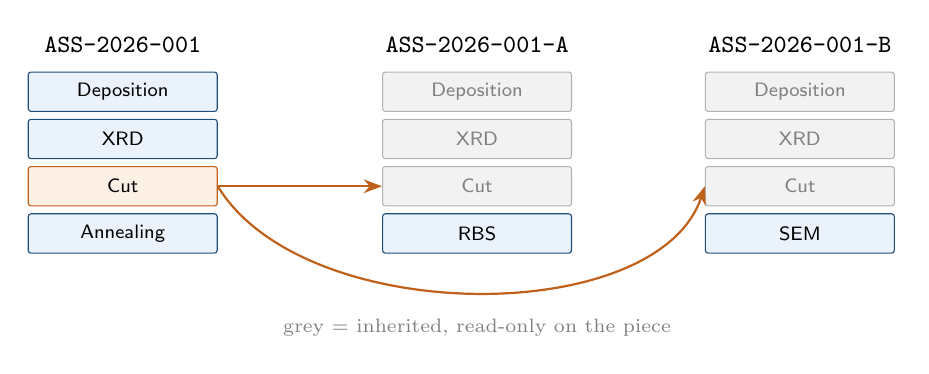
\begin{tikzpicture}[
  ent/.style={draw=accent,fill=tipbg,rounded corners=1pt,minimum width=2.4cm,
              minimum height=0.5cm,font=\sffamily\scriptsize},
  inh/.style={ent,draw=gray!60,fill=gray!10,text=gray},
  cut/.style={ent,fill=warnbg,draw=warnfr},
  lbl/.style={font=\sffamily\small\bfseries}]
  % parent
  \node[lbl] at (0,0.6) {\sid{ASS-2026-001}};
  \node[ent] (p1) at (0,0) {Deposition};
  \node[ent] (p2) at (0,-0.6) {XRD};
  \node[cut] (p3) at (0,-1.2) {Cut};
  \node[ent] (p4) at (0,-1.8) {Annealing};
  % piece A
  \node[lbl] at (4.5,0.6) {\sid{ASS-2026-001-A}};
  \node[inh] at (4.5,0) {Deposition};
  \node[inh] at (4.5,-0.6) {XRD};
  \node[inh] (a3) at (4.5,-1.2) {Cut};
  \node[ent] at (4.5,-1.8) {RBS};
  % piece B
  \node[lbl] at (8.6,0.6) {\sid{ASS-2026-001-B}};
  \node[inh] at (8.6,0) {Deposition};
  \node[inh] at (8.6,-0.6) {XRD};
  \node[inh] (b3) at (8.6,-1.2) {Cut};
  \node[ent] at (8.6,-1.8) {SEM};
  \draw[-{Stealth},thick,warnfr] (p3.east) -- (a3.west);
  \draw[-{Stealth},thick,warnfr] (p3.east) .. controls (2.3,-3.0) and (6.8,-3.0) .. (b3.west);
  \node[font=\scriptsize,text=gray] at (4.5,-3.0) {grey = inherited, read-only on the piece};
\end{tikzpicture}
\end{center}

Each piece:
\begin{itemize}
  \item \textbf{inherits} the parent's timeline up to the Cut step, shown
        greyed out with ``from \ldots''. Nothing is copied: correcting an
        entry on the parent corrects it for every piece. Inherited entries
        are edited on the parent.
  \item copies the parent's type, substrate, film, tags and sharing.
  \item gets its own entries after the cut, separate from its siblings.
\end{itemize}

The parent stays usable; what you add to it afterwards belongs to the
parent only. Whoever can see a piece also sees its inherited history.

%=====================================================================
\section{Sharing and ownership}
%=====================================================================

\subsection{Sharing a sample}

On a sample's page, in the \ui{Sharing} panel, choose \ui{Share with\ldots},
pick a person and \ui{View} or \ui{Edit}:

\begin{description}
  \item[View] Read the details and download files.
  \item[Edit] Also add and change steps, analyses and files.
\end{description}

To share many samples at once, go to \menu{Search}, tick the samples (or
\ui{select all mine}) and use \ui{Share selected samples with}. Only the
owner or an administrator can change sharing or delete a sample.

\subsection{Performed by}

Listing someone under \ui{Performed by} lets them see and edit that one
entry (and its photos and files) even without access to the rest of the
sample. They are told by email. This is the easiest way to let the
technician who ran the XRD upload the data.

\subsection{Giving a sample to someone else}
\label{sec:assign}

You can make another researcher the owner:
\begin{itemize}
  \item on the \menu{New Sample} form (the ID then uses their initials);
  \item on the sample's \ui{Edit} form;
  \item per piece on the cut form.
\end{itemize}

Unless an administrator does it, the new owner has to confirm. They get
an email and see the sample under \emph{Assigned to you --- please confirm}
on the \menu{Samples} page, where they can \ui{Accept} or \ui{Decline} (which
gives it back). Until then, and afterwards, whoever assigned it keeps edit
access.

%=====================================================================
\section{Substrates and projects}
%=====================================================================

\subsection{Substrate library}

The \menu{Substrates} tab lists substrates with material, thickness,
orientation, polishing, size, supplier, notes and spec files. Anyone can
add one; whoever added it and administrators can edit it. A substrate used
by a sample can't be deleted.

\subsection{Projects}

The \menu{Projects} tab lists collaborations: name, partner institution,
code, country, contact and notes. The code (2--6 letters or digits) is used
in the IDs of the project's samples, so it can't match anyone's initials,
and it is fixed once a sample uses it. An institution can have several
projects; pick it from the suggestions so it's always spelled the same way.

%=====================================================================
\section{Search and export}
%=====================================================================

\menu{Search} filters samples by free text, researcher, sample type,
material, technique and tag, and groups the results (by
researcher, year, type, material, technique, tag or project). Free text
matches IDs, labels, descriptions, notes, parameters and project names, but only on
samples whose details you can see.

\ui{Export results (CSV)} downloads the matching samples, with one row per
step or analysis and one \texttt{param:\ldots} column per parameter. It
opens in Excel, Origin or Python (\texttt{pandas.read\_csv}). Details are
left blank for samples you can't view.

%=====================================================================
\section{Suggestions}
%=====================================================================

The \menu{Suggestions} tab is for anything: a bug, a missing field, a new
dropdown value you can't add, an idea. It records which page you were on.
Administrators reply there; you'll see a badge when they do, and you can
answer back.

%=====================================================================
\section{For administrators}
\label{sec:admin}
%=====================================================================

\menu{Configurations} has three parts.

\begin{description}
  \item[Users] Create accounts (a temporary password is emailed, or shown on
    screen if email isn't set up), reset passwords, make or remove
    administrators, change someone's name or initials, delete users.
  \item[Process Step Types / Analysis Types] Add, edit or delete (when
    unused) types. Each has a \emph{parameter schema}: a JSON list of fields.
    Editing it never changes stored data.
  \item[Export full database (CSV)] Everything, regardless of sharing.
\end{description}

The \menu{Inbox} collects everyone's suggestions; reply, and mark them
solved or reopen them.

\subsection{Parameter schemas}

Each field has a \texttt{key}, a \texttt{label} and a \texttt{type}:

\begin{center}
\small
\begin{tabularx}{\linewidth}{@{}l>{\raggedright}p{4cm}X@{}}
\toprule
\textbf{type} & \textbf{entered as} & \textbf{extra keys} \\
\midrule
\texttt{number}   & a number box & \texttt{unit}, \texttt{placeholder} \\
\texttt{duration} & \texttt{min:s}, \texttt{h:min:s} or minutes & \texttt{unit}, \texttt{placeholder} \\
\texttt{text}     & a one-line box & \texttt{placeholder} \\
\texttt{longtext} & a large box & \texttt{placeholder} \\
\texttt{choice}   & a shared dropdown & \texttt{list}; \texttt{located: true} for equipment \\
\texttt{variant}  & pick one option, each with its own fields & \texttt{options} \\
\texttt{check}    & a tick box revealing fields & \texttt{fields} \\
\texttt{modes}    & tick several; each gets the same fields & \texttt{list}, \texttt{fields} \\
\bottomrule
\end{tabularx}
\end{center}

Example (Annealing):

\begin{tcolorbox}[colback=gray!5,colframe=gray!40,boxrule=0.4pt,arc=1pt]
\footnotesize
\begin{verbatim}
[{"key": "method", "label": "Method", "type": "variant", "options": [
   {"value": "Furnace", "fields": [
     {"key": "temperature", "label": "Temperature", "type": "number", "unit": "°C"},
     {"key": "duration", "label": "Duration", "type": "number", "unit": "min"}]},
   {"value": "RTA", "fields": [
     {"key": "atmosphere", "label": "Atmosphere", "type": "choice", "list": "atmosphere"},
     {"key": "temperature", "label": "Temperature", "type": "number", "unit": "°C"},
     {"key": "duration", "label": "Duration", "type": "number", "unit": "s"},
     {"key": "ramp", "label": "Ramp", "type": "number", "unit": "°C/s"}]}]}]
\end{verbatim}
\end{tcolorbox}

%=====================================================================
\section{Running the server}
\label{sec:install}
%=====================================================================

The full details are in the repository's \texttt{README.md}. In short:

\begin{tcolorbox}[colback=gray!5,colframe=gray!40,boxrule=0.4pt,arc=1pt]
\footnotesize
\begin{verbatim}
cp .env.example .env          # set SECRET_KEY, BASE_URL, SMTP_PASSWORD
docker compose up -d
docker compose exec app python -m backend.create_admin
\end{verbatim}
\end{tcolorbox}

\subsection{What to back up}

\begin{center}
\begin{tabular}{@{}ll@{}}
\toprule
Database (samples, timelines, users) & the \texttt{pgdata} Docker volume \\
Photos and data files                & the \texttt{uploads/} folder \\
Settings and passwords               & \texttt{.env} \\
\bottomrule
\end{tabular}
\end{center}

\begin{tcolorbox}[colback=gray!5,colframe=gray!40,boxrule=0.4pt,arc=1pt]
\footnotesize
\begin{verbatim}
docker compose exec -T db pg_dump -U logbook logbook > backup_$(date +%Y%m%d).sql
\end{verbatim}
\end{tcolorbox}

Keep the dump together with a copy of \texttt{uploads/}. That folder
has one subfolder per sample ID and, inside it, one per step or analysis,
with the files under their original names (e.g.\
\nolinkurl{ASS-2026-001/2026-10-22_XRD-HRXRD/scan01.raw}), but it's the
database that links each file to its entry.

\begin{careful}
\texttt{docker compose down} stops the logbook and keeps the data.
\texttt{docker compose down -v} \textbf{deletes the database}.
\end{careful}

\end{document}
